\documentclass{article}
\usepackage[UTF8]{ctex}
\usepackage[T1]{fontenc}
\usepackage[utf8]{inputenc}
\usepackage{titlesec}
\usepackage[colorlinks, linkcolor = black]{hyperref}
\usepackage{float}
\usepackage{xcolor}
\usepackage{tikz}
\usepackage{amsmath}
\usepackage{subfigure}
\usetikzlibrary{positioning}
\usetikzlibrary[arrows, shapes, chains]
\newcounter{row}
\newcounter{col}

\newcommand\setrow[3]{
  \setcounter{col}{1}
  \foreach \n in {#1, #2, #3} {
    \edef\x{\value{col} - 0.5}
    \edef\y{3.5 - \value{row}}
    \node[anchor = center] at (\x, \y) {\n};
    \stepcounter{col}
  }
  \stepcounter{row}
}
\titleformat{\section}[block]{\LARGE\scshape}{\arabic{section}}{1em}{}[]

\tikzset{
    state/.style = {text ragged},
    terminal/.style = {rectangle, draw = black, text ragged},
    loop/.style = {rectangle, draw = black, double, text ragged},
    value/.style = {circle, draw = black, text ragged, minimum width = 2em, scale = 0.7},
    level distance = 3em
}

\title{Homework 3}
\author{PB17000297 罗晏宸}
\date{March 16 2020}

\begin{document}
\maketitle

\section{Exercise 5.8}
考虑图\ref{figure5.17}中描述的两人游戏。
\begin{figure}[h]
    {
        \centering
        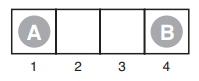
\includegraphics[]{Figure5-17.png}
        \caption{一个简单游戏的初始棋局}
        \label{figure5.17}
    }
    选手\textit{A}先走。两个选手轮流走棋,每个人必须把自己的棋子移动到任一方向上的相邻空位中。如果对方的棋子占据着相邻的位置,你可以跳过对方的棋子到下一个空位。(例如,\textit{A}在位置3,\textit{B}在位置2,那么\textit{A}可以移回1。)当一方的棋子移动到对方的端点时游戏结束。如果 \textit{A} 先到达位置4,\textit{A}的值为$+1$;如果\textit{B}先到达位置1,\textit{A}的值为$-1$。
\end{figure}
\subparagraph{a}
根据如下约定画出完整博弈树:
\begin{itemize}
    \item 每个状态用$(s_A,\, s_B)$表示,其中$s_A$和$s_B$表示棋子的位置。
    \item 每个终止状态用方框画出,用圆圈写出它的博弈值。
    \item 把循环状态(在到根结点的路径上已经出现过的状态)画上双层方框。由于不清楚他们的值,在圆圈里标记一个“?”。
\end{itemize}
\subparagraph{b}
给出每个结点倒推的极小极大值(也标记在圆圈里)。解释怎样处理“?”值和为什么这么处理。
\subparagraph{c}
解释标准的极小极大算法为什么在这棵博弈树中会失败,简要说明你将如何修正它,在(b)的图上画出你的答案。你修正后的算法对于所有包含循环的游戏都能给出最优决策吗?
\subparagraph{d}
这个4-方格游戏可以推广到$n$个方格,其中$n > 2$。证明如果$n$是偶数\textit{A}一定能赢,而$n$是奇数则\textit{A}一定会输。

\paragraph{解}
\subparagraph{a}
博弈树如图\ref{figureTree}所示
\begin{figure}[h]
    \centering
    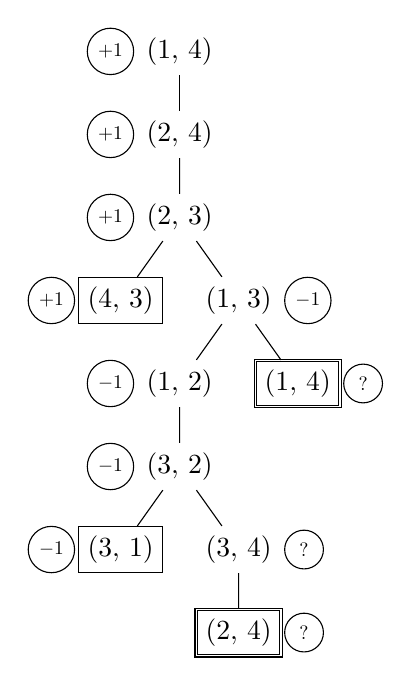
\begin{tikzpicture}
        \node [state] (1) {$(1,\, 4)$}
            child {node [state] (2) {$(2,\, 4)$}
                child {node [state] (3) {$(2,\, 3)$}
                    child {node [terminal] (4) {$(4,\, 3)$}}
                    child {node [state] (5) {$(1,\, 3)$}
                        child {node [state] (6) {$(1,\, 2)$}
                            child {node [state] (8) {$(3,\, 2)$}
                                child {node [terminal] (9) {$(3,\, 1)$}}
                                child {node [state] (10) {$(3,\, 4)$}
                                    child {node [loop] (11) {$(2,\, 4)$}}
                                }
                            }
                        }
                        child {node [loop] (7) {$(1,\, 4)$}}
                    }
                }
            };
        \node [value, left = 0.1em of 1] (v1) {$+1$};
        \node [value, left = 0.1em of 2] (v2) {$+1$};
        \node [value, left = 0.1em of 3] (v3) {$+1$};
        \node [value, left = 0.1em of 4] (v4) {$+1$};
        \node [value, right = 0.1em of 5] (v5) {$-1$};
        \node [value, left = 0.1em of 6] (v6) {$-1$};
        \node [value, right = 0.1em of 7] (v7) {$?$};
        \node [value, left = 0.1em of 8] (v8) {$-1$};
        \node [value, left = 0.1em of 9] (v9) {$-1$};
        \node [value, right = 0.1em of 10] (v10) {$?$};
        \node [value, right = 0.1em of 11] (v11) {$?$};
    \end{tikzpicture}
    \caption{两人游戏的博弈树}
    \label{figureTree}
\end{figure}

\subparagraph{b}
在圆圈中的博弈值后附上相应的极小与极大值,如图\ref{figureTree2}所示
\begin{figure}
    \centering
    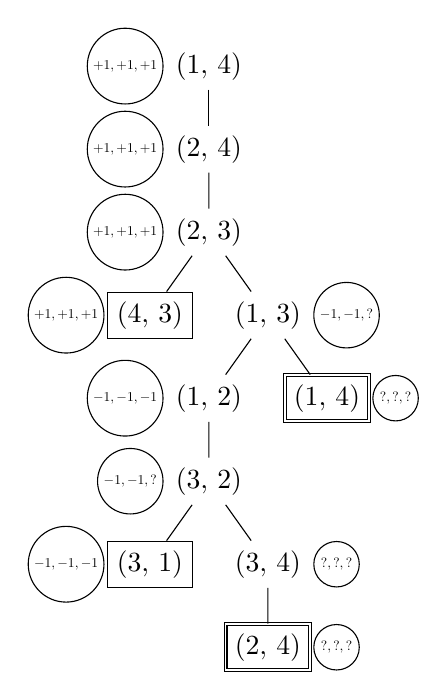
\begin{tikzpicture}
        \node [state] (1) {$(1,\, 4)$}
            child {node [state] (2) {$(2,\, 4)$}
                child {node [state] (3) {$(2,\, 3)$}
                    child {node [terminal] (4) {$(4,\, 3)$}}
                    child {node [state] (5) {$(1,\, 3)$}
                        child {node [state] (6) {$(1,\, 2)$}
                            child {node [state] (8) {$(3,\, 2)$}
                                child {node [terminal] (9) {$(3,\, 1)$}}
                                child {node [state] (10) {$(3,\, 4)$}
                                    child {node [loop] (11) {$(2,\, 4)$}}
                                }
                            }
                        }
                        child {node [loop] (7) {$(1,\, 4)$}}
                    }
                }
            };
        \node [value, scale = 0.7, left = 0.1em of 1] (v1) {$+1, +1, +1$};
        \node [value, scale = 0.7, left = 0.1em of 2] (v2) {$+1, +1, +1$};
        \node [value, scale = 0.7, left = 0.1em of 3] (v3) {$+1, +1, +1$};
        \node [value, scale = 0.7, left = 0.1em of 4] (v4) {$+1, +1, +1$};
        \node [value, scale = 0.7, right = 0.1em of 5] (v5) {$-1, -1, ?$};
        \node [value, scale = 0.7, left = 0.1em of 6] (v6) {$-1, -1, -1$};
        \node [value, scale = 0.7, right = 0.1em of 7] (v7) {$?, ?, ?$};
        \node [value, scale = 0.7, left = 0.1em of 8] (v8) {$-1, -1, ?$};
        \node [value, scale = 0.7, left = 0.1em of 9] (v9) {$-1, -1, -1$};
        \node [value, scale = 0.7, right = 0.1em of 10] (v10) {$?, ?, ?$};
        \node [value, scale = 0.7, right = 0.1em of 11] (v11) {$?, ?, ?$};
    \end{tikzpicture}
    \caption{标注每个结点倒推极小极大值的博弈树}
    \label{figureTree2}
\end{figure}
对于“?”值采取的处理办法是,如果Agent能够选择则总是会选择获胜(即博弈值为$+1$),因此除非后继结点均为“?”,可以将“?”视为介于$-1$与$+1$之间的值。
\subparagraph{c}
标准的极小极大算法是深度优先的,会在遇到循环状态时陷入无限循环。一个可行的修正方式是带记录的深度优先搜索,通过维护一个队列记录已遍历的结点,如果遇到已在队列中的重复状态,就直接返回“?”,通过前述的处理方法来解决比较。答案如所示。
\begin{figure}[h]
    \centering
    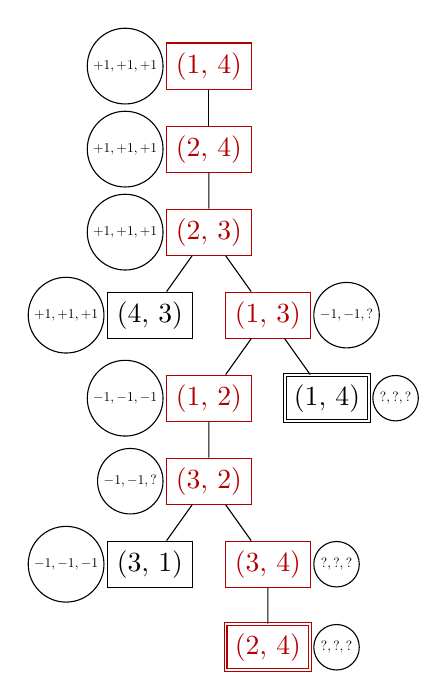
\begin{tikzpicture}
        \node [state, draw = red!70!black, red!70!black] (1) {$(1,\, 4)$}
            child {node [state, draw = red!70!black, red!70!black] (2) {$(2,\, 4)$}
                child {node [state, draw = red!70!black, red!70!black] (3) {$(2,\, 3)$}
                    child {node [terminal] (4) {$(4,\, 3)$}}
                    child {node [state, draw = red!70!black, red!70!black] (5) {$(1,\, 3)$}
                        child {node [state, draw = red!70!black, red!70!black] (6) {$(1,\, 2)$}
                            child {node [state, draw = red!70!black, red!70!black] (8) {$(3,\, 2)$}
                                child {node [terminal] (9) {$(3,\, 1)$}}
                                child {node [state, draw = red!70!black, red!70!black] (10) {$(3,\, 4)$}
                                    child {node [loop, draw = red!70!black, red!70!black] (11) {$(2,\, 4)$}}
                                }
                            }
                        }
                        child {node [loop] (7) {$(1,\, 4)$}}
                    }
                }
            };
        \node [value, scale = 0.7, left = 0.1em of 1] (v1) {$+1, +1, +1$};
        \node [value, scale = 0.7, left = 0.1em of 2] (v2) {$+1, +1, +1$};
        \node [value, scale = 0.7, left = 0.1em of 3] (v3) {$+1, +1, +1$};
        \node [value, scale = 0.7, left = 0.1em of 4] (v4) {$+1, +1, +1$};
        \node [value, scale = 0.7, right = 0.1em of 5] (v5) {$-1, -1, ?$};
        \node [value, scale = 0.7, left = 0.1em of 6] (v6) {$-1, -1, -1$};
        \node [value, scale = 0.7, right = 0.1em of 7] (v7) {$?, ?, ?$};
        \node [value, scale = 0.7, left = 0.1em of 8] (v8) {$-1, -1, ?$};
        \node [value, scale = 0.7, left = 0.1em of 9] (v9) {$-1, -1, -1$};
        \node [value, scale = 0.7, right = 0.1em of 10] (v10) {$?, ?, ?$};
        \node [value, scale = 0.7, right = 0.1em of 11] (v11) {$?, ?, ?$};
    \end{tikzpicture}
    \caption{修正后求解两人游戏的答案}
\end{figure}
修正后的算法并不能给出所有包含循环的游戏的最优决策,因为这样的处理方法不能区分不同的“?”值,在获胜情况并不唯一,或者有不同获胜程度的状态时,直接返回可能会丢失其他获胜程度较深的状态。
\subparagraph{d}
当$n = 3$和$n = 4$时,\textit{A}分别输掉和赢得游戏,很显然对于$n \geq 4$的情况,\textit{A}和\textit{B}在开始都会向对方走一格,如果\textit{A}在$n - 2$的情况获胜,那么在这种情况(\textit{A}处于位置1,\textit{B}处于位置$n - 1$)下,\textit{A}将会在\textit{B}到达位置1之前到达位置$n - 1$,那么\textit{A}也将会在$n$的情况下获胜,在这种情况下\textit{A}不会向着自己的原始位置行棋;同理如果\textit{A}在$n - 2$的情况失败,意味着\textit{B}获胜,那么\textit{B}也将会在$n$的情况获胜。因此如果$n$是偶数\textit{A}一定能赢,而$n$是奇数则\textit{A}一定会输。

\section{Exercise 5.9}
本题以井字棋(圈与十字游戏)为例练习博弈中的基本概念。定义$X_n$为恰好有$n$个$X$而没有$O$的行、列或者对角线的数目。同样$O_n$为正好有$n$个$O$的行、列或者对角线的数目。效用函数给$X_3 = 1$的棋局$+1$,给$O_3 = 1$的棋局$-1$。所有其他终止状态效用值为0。对于非终止状态,使用线性的评估函数定义为$\textit{Eval}(s) = 3X_2(s) + X_1(s) - (3O_2(s) + O_1(s))$。
\subparagraph{a}
估算可能的井字棋局数。
\subparagraph{b}
考虑对称性,给出从空棋盘开始的深度为2的完整博弈树(即,在棋盘上一个$X$一个$O$的棋局)。
\subparagraph{c}
标出深度为2的棋局的评估函数值。
\subparagraph{d}
使用极小极大算法标出深度为1和0的棋局的倒推值,并根据这些值选出最佳的起始行棋。
\subparagraph{e}
假设结点按对$\alpha$-$\beta$剪枝的最优顺序生成,圈出使用$\alpha$-$\beta$剪枝将被剪掉的深度为2的结点。

\paragraph{解}
\subparagraph{a}
井字棋最多可能将棋盘的9个格子下满,最少需要双方轮流执棋两合后先手获胜,因此可能的局数在$\frac{9!}{4!}$到$9!$之间。

\subparagraph{b}
完整博弈树如图\ref{figureDeep2}所示
\begin{figure}[h]
    \centering
    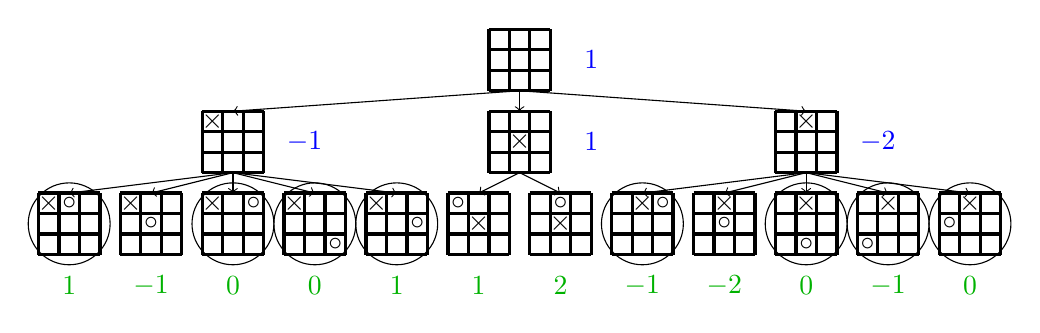
\begin{tikzpicture}[scale = 1.3]
        \begin{scope}[scale = 0.2]
            \draw[very thick] (0, 0) grid (3, 3);
            \setcounter{row}{1}
            \setrow { }{ }{ }
            \setrow { }{ }{ }
            \setrow { }{ }{ }
        \end{scope}
        \begin{scope}[scale = 0.2, xshift = -14cm, yshift = -4cm]
            \draw[very thick] (0, 0) grid (3, 3);
            \setcounter{row}{1}
            \setrow {$\times$}{ }{ }
            \setrow { }{ }{ }
            \setrow { }{ }{ }
        \end{scope}
        \begin{scope}[scale = 0.2, yshift = -4cm]
            \draw[very thick] (0, 0) grid (3, 3);
            \setcounter{row}{1}
            \setrow { }{ }{ }
            \setrow { }{$\times$}{ }
            \setrow { }{ }{ }
        \end{scope}
        \begin{scope}[scale = 0.2, xshift = 14cm, yshift = -4cm]
            \draw[very thick] (0, 0) grid (3, 3);
            \setcounter{row}{1}
            \setrow { }{$\times$}{ }
            \setrow { }{ }{ }
            \setrow { }{ }{ }
        \end{scope}
        \begin{scope}[scale = 0.2, xshift = -22cm, yshift = -8cm]
            \draw[very thick] (0, 0) grid (3, 3);
            \setcounter{row}{1}
            \setrow {$\times$}{$\circ$}{ }
            \setrow { }{ }{ }
            \setrow { }{ }{ }
        \end{scope}
        \begin{scope}[scale = 0.2, xshift = -18cm, yshift = -8cm]
            \draw[very thick] (0, 0) grid (3, 3);
            \setcounter{row}{1}
            \setrow {$\times$}{ }{ }
            \setrow { }{$\circ$}{ }
            \setrow { }{ }{ }
        \end{scope}
        \begin{scope}[scale = 0.2, xshift = -14cm, yshift = -8cm]
            \draw[very thick] (0, 0) grid (3, 3);
            \setcounter{row}{1}
            \setrow {$\times$}{ }{$\circ$}
            \setrow { }{ }{ }
            \setrow { }{ }{ }
        \end{scope}
        \begin{scope}[scale = 0.2, xshift = -10cm, yshift = -8cm]
            \draw[very thick] (0, 0) grid (3, 3);
            \setcounter{row}{1}
            \setrow {$\times$}{ }{ }
            \setrow { }{ }{ }
            \setrow { }{ }{$\circ$}
        \end{scope}
        \begin{scope}[scale = 0.2, xshift = -6cm, yshift = -8cm]
            \draw[very thick] (0, 0) grid (3, 3);
            \setcounter{row}{1}
            \setrow {$\times$}{ }{ }
            \setrow { }{ }{$\circ$}
            \setrow { }{ }{ }
        \end{scope}
        \begin{scope}[scale = 0.2, xshift = -2cm, yshift = -8cm]
            \draw[very thick] (0, 0) grid (3, 3);
            \setcounter{row}{1}
            \setrow {$\circ$}{ }{ }
            \setrow { }{$\times$}{ }
            \setrow { }{ }{ }
        \end{scope}
        \begin{scope}[scale = 0.2, xshift = 2cm, yshift = -8cm]
            \draw[very thick] (0, 0) grid (3, 3);
            \setcounter{row}{1}
            \setrow { }{$\circ$}{ }
            \setrow { }{$\times$}{ }
            \setrow { }{ }{ }
        \end{scope}
        \begin{scope}[scale = 0.2, xshift = 6cm, yshift = -8cm]
            \draw[very thick] (0, 0) grid (3, 3);
            \setcounter{row}{1}
            \setrow { }{$\times$}{$\circ$}
            \setrow { }{ }{ }
            \setrow { }{ }{ }
        \end{scope}
        \begin{scope}[scale = 0.2, xshift = 10cm, yshift = -8cm]
            \draw[very thick] (0, 0) grid (3, 3);
            \setcounter{row}{1}
            \setrow { }{$\times$}{ }
            \setrow { }{$\circ$}{ }
            \setrow { }{ }{ }
        \end{scope}
        \begin{scope}[scale = 0.2, xshift = 14cm, yshift = -8cm]
            \draw[very thick] (0, 0) grid (3, 3);
            \setcounter{row}{1}
            \setrow { }{$\times$}{ }
            \setrow { }{ }{ }
            \setrow { }{$\circ$}{ }
        \end{scope}
        \begin{scope}[scale = 0.2, xshift = 18cm, yshift = -8cm]
            \draw[very thick] (0, 0) grid (3, 3);
            \setcounter{row}{1}
            \setrow { }{$\times$}{ }
            \setrow { }{ }{ }
            \setrow {$\circ$}{ }{ }
        \end{scope}
        \begin{scope}[scale = 0.2, xshift = 22cm, yshift = -8cm]
            \draw[very thick] (0, 0) grid (3, 3);
            \setcounter{row}{1}
            \setrow { }{$\times$}{ }
            \setrow {$\circ$}{ }{ }
            \setrow { }{ }{ }
        \end{scope}
        \draw [->] (0.3, 0) to (0.3, -0.2);
        \draw [->] (0.3, 0) to (-2.5, -0.2);
        \draw [->] (0.3, 0) to (3.1, -0.2);
        \draw [->] (-2.5, -0.8) to (-4.1, -1.0);
        \draw [->] (-2.5, -0.8) to (-3.3, -1.0);
        \draw [->] (-2.5, -0.8) to (-2.5, -1.0);
        \draw [->] (-2.5, -0.8) to (-1.7, -1.0);
        \draw [->] (-2.5, -0.8) to (-0.9, -1.0);
        \draw [->] (0.3, -0.8) to  (-0.1, -1.0);
        \draw [->] (0.3, -0.8) to  ( 0.7, -1.0);
        \draw [->] (3.1, -0.8) to  ( 1.5, -1.0);
        \draw [->] (3.1, -0.8) to  ( 2.3, -1.0);
        \draw [->] (3.1, -0.8) to  ( 3.1, -1.0);
        \draw [->] (3.1, -0.8) to  ( 3.9, -1.0);
        \draw [->] (3.1, -0.8) to  ( 4.7, -1.0);

        \node [green!70!black] at (-4.1, -1.9) {$1$};
        \node [green!70!black] at (-3.3, -1.9) {$-1$};
        \node [green!70!black] at (-2.5, -1.9) {$0$};
        \node [green!70!black] at (-1.7, -1.9) {$0$};
        \node [green!70!black] at (-0.9, -1.9) {$1$};
        \node [green!70!black] at (-0.1, -1.9) {$1$};
        \node [green!70!black] at ( 0.7, -1.9) {$2$};
        \node [green!70!black] at ( 1.5, -1.9) {$-1$};
        \node [green!70!black] at ( 2.3, -1.9) {$-2$};
        \node [green!70!black] at ( 3.1, -1.9) {$0$};
        \node [green!70!black] at ( 3.9, -1.9) {$-1$};
        \node [green!70!black] at ( 4.7, -1.9) {$0$};

        \node [blue] at (1.0, 0.3) {$1$};
        \node [blue] at (-1.8, -0.5) {$-1$};
        \node [blue] at (1.0, -0.5) {$1$};
        \node [blue] at (3.8, -0.5) {$-2$};

        \draw (-4.1, -1.3) circle [radius = 0.4];
        \draw (-2.5, -1.3) circle [radius = 0.4];
        \draw (-1.7, -1.3) circle [radius = 0.4];
        \draw (-0.9, -1.3) circle [radius = 0.4];
        \draw ( 1.5, -1.3) circle [radius = 0.4];
        \draw ( 3.1, -1.3) circle [radius = 0.4];
        \draw ( 3.9, -1.3) circle [radius = 0.4];
        \draw ( 4.7, -1.3) circle [radius = 0.4];

    \end{tikzpicture}
    \caption{从空棋盘开始的深度为2的完整博弈树}
    \label{figureDeep2}
\end{figure}

\subparagraph{c}
评估函数值已在图\ref{figureDeep2}中以{\color{green!70!black} 绿色}标出

\subparagraph{d}
倒推值已在图\ref{figureDeep2}中以{\color{blue} 蓝色}标出,可知最佳的起始行棋是在棋盘中央落子。

\subparagraph{e}
被剪掉的结点已在图\ref{figureDeep2}中圈出。

\section{Exercise 5.13}
请给出$\alpha$-$\beta$剪枝正确性的形式化证明。要做到这一点需考虑图\ref{figure5.18}。问题为是否要剪掉结点$n_j$,它是一个MAX结点,是$n_1$的一个后代。基本的思路是当且仅当$n_1$的极小极大值可以被证明独立于$n_j$的值时,会发生剪枝。
\begin{figure}[h]
    {
        \centering
        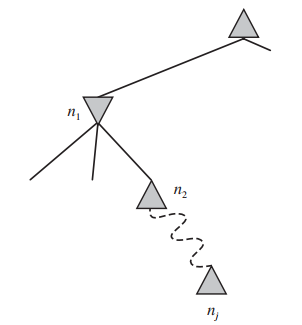
\includegraphics[]{Figure5-18.png}
        \caption{是否剪掉结点$n_j$时的情形}
        \label{figure5.18}
    }
\end{figure}
\subparagraph{a}
$n_1$的值时所有后代结点的最小值:$n_1 = \min(n_2,\, n_{2\,1},\, \cdots,\, n_{2\,b_2})$。请为$n_2$找到类似的表达式,以得到用$n_j$表示的$n_1$的表达式。
\subparagraph{b}
深度为$i$的结点$n_i$的极小极大值已知,$l_i$是在结点$n_i$左侧结点的极小值(或者极大值)。同样,$r_i$是在$n_i$右侧的未探索过的结点的极小值(或者极大值)。用$l_i$和$r_i$的值重写$n_1$的表达式。
\subparagraph{c}
现在重新形式化表达式,来说明为了向$n_1$施加影响,$n_j$不能超出有$l_i$值得到的某特定界限。
\subparagraph{d}
假设$n_j$是MIN结点的情况,请重复上面的过程。

\paragraph{解}
\subparagraph{a}
类似的,有$n_2 = \max(n_3,\, n_{3\,1},\, \cdots,\, n_{3\,b_3})$,得到
\begin{equation*}
    n_1 = \min(\max( \cdots \max(n_j,\, n_{j\,1},\, \cdots,\, n_{j\,b_j})),\, n_{2\,1},\, \cdots,\, n_{2\,b_2})
\end{equation*}

\subparagraph{b}
改写$n_1$如下
\begin{align*}
    n_1 &= \min(l_2,\, n_2,\, r_2) \\
    &= \min(l_2,\, \max(l_3,\, n_3,\, r_3),\, r_2) \\
    &\vdots \\
    &= \min(l_2,\, \max(l_3,\, \max( \cdots \max(l_j,\, n_j,\, r_j),\, \cdots),\, r_3),\, r_2)
\end{align*}

\subparagraph{c}
由前述可知
\begin{equation*}
    n_i = \min(l_{i + 1},\, \max(l_{i + 2},\, \max( \cdots \max(l_j,\, n_j,\, r_j),\, \cdots),\, r_{i + 2}),\, r_{i + 1})
\end{equation*}
由于$n_j$是一个MAX结点,为了向$n_1$施加影响,$n_j$不能超出$\min(l_2,\, l_4,\, \cdots,\, l_j)$。

\subparagraph{d}
假设$n_j$是MIN结点,只需要交换前述中的$\max$与$\min$即可。
\end{document}